\chapter{Phân tích, thiết kế và triển khai hệ thống TMAP}

\section{Phân tích Yêu cầu Hệ thống}

Hệ thống TMAP hướng đến phục vụ hai nhóm đối tượng chính: \textbf{Người sáng tạo nội dung} (sử dụng Trình biên soạn) và \textbf{Người trải nghiệm} (sử dụng Ứng dụng di động). Việc phân tích yêu cầu được thực hiện theo từng nhóm đối tượng để đảm bảo các chức năng được xây dựng đáp ứng đúng mục tiêu đã đặt ra tại Chương 1.

\subsection{Yêu cầu Chức năng}

Các yêu cầu chức năng được hệ thống TMAP phải đáp ứng được tóm tắt trong \tablename~\ref{tab:YeuCauChucNang}.
\begin{table}[h]
    \centering
    \caption{Tóm tắt các yêu cầu chức năng của hệ thống TMAP}
    \label{tab:YeuCauChucNang}
    \resizebox{\textwidth}{!}{
    \begin{tabular}{|c|p{10cm}|}
        \hline
        \textbf{Thành phần} & \textbf{Mô tả Yêu cầu} \\
        \hline
        Editor & Quản lý vòng đời của Map (Tạo mới, Chỉnh sửa, Xóa, Xuất bản Map). \\
        \hline
        Editor & Định vị địa lý: Cho phép chọn và ghi lại tọa độ chính xác của các Điểm tham quan (POI) trên giao diện bản đồ tích hợp. \\
        \hline
        Editor & Xây dựng tuyến: Cho phép thiết lập và thay đổi thứ tự tham quan rõ ràng giữa các POI trong một Map. \\
        \hline
        Editor & Quản lý nội dung: Hỗ trợ tải lên và biên tập nội dung đa phương tiện (văn bản, hình ảnh, video, audio) cho mỗi POI. \\
        \hline
        Editor & Thiết lập tương tác: Cho phép người tạo cấu hình các hoạt động tương tác tại POI (ví dụ: trắc nghiệm, yêu cầu chụp ảnh, ghi âm, nhận xét văn bản). \\
        \hline
        Player & Xác thực người dùng: Hỗ trợ đăng ký, đăng nhập và quản lý hồ sơ cá nhân. \\
        \hline
        Player & Tìm kiếm và Truy cập Map: Hiển thị danh sách các Map đã xuất bản và cho phép tìm kiếm theo tên/vị trí. \\
        \hline
        Player & Định vị thực địa: Sử dụng GPS để xác định và hiển thị vị trí hiện tại của du khách và các POI trên bản đồ. \\
        \hline
        Player & Hướng dẫn lộ trình: Dẫn dắt du khách đi theo thứ tự đã định và đánh dấu trạng thái hoàn thành của POI. \\
        \hline
        Player & Thực hiện Tương tác: Cung cấp giao diện để người dùng tham gia vào hoạt động tương tác theo yêu cầu của Editor khi đến POI. \\
        \hline
        Player & Lưu trữ kết quả: Ghi lại và bảo mật kết quả tương tác của người dùng trên hệ thống thông qua API. \\
        \hline
    \end{tabular}
    }
\end{table}

\begin{enumerate}
    \item \textbf{Đối với Trình biên soạn Web (Editor):}
    \begin{itemize}
        \item Quản lý Map: Cho phép người dùng tạo mới, chỉnh sửa, xóa và xuất bản các Map trải nghiệm.
        \item Định vị địa lý: Cung cấp giao diện tích hợp Google Maps để chọn và định vị chính xác tọa độ của từng điểm tham quan trên bản đồ.
        \item Xây dựng tuyến: Cho phép thiết lập thứ tự và lộ trình tham quan giữa các điểm một cách rõ ràng.
        \item Quản lý nội dung: Hỗ trợ tải lên và biên tập nội dung mô tả đa phương tiện (văn bản, hình ảnh, video, audio) cho mỗi điểm.
        \item Thiết lập tương tác: Cho phép người dùng cấu hình các hoạt động tương tác tại điểm tham quan (ví dụ: trắc nghiệm, chụp ảnh, ghi âm, nhận xét văn bản).
    \end{itemize}

    \item \textbf{Đối với Ứng dụng trải nghiệm di động (Player):}
    \begin{itemize}
        \item Xác thực người dùng: Quản lý việc đăng ký, đăng nhập và bảo mật thông tin người dùng.
        \item Tìm kiếm và Truy cập Map: Hiển thị danh sách các Map đã được xuất bản và cung cấp chức năng tìm kiếm, lọc theo tiêu chí.
        \item Định vị thực địa: Sử dụng GPS để xác định vị trí hiện tại của du khách và hiển thị vị trí của các điểm tham quan trên bản đồ.
        \item Hướng dẫn lộ trình: Dẫn dắt du khách đi theo thứ tự đã định, đánh dấu các điểm đã hoàn thành.
        \item Thực hiện Tương tác: Cung cấp giao diện để người dùng tham gia vào các hoạt động tương tác và lưu trữ kết quả tương tác đó.
    \end{itemize}
\end{enumerate}

\subsection{Yêu cầu Phi Chức năng}

Ngoài các yêu cầu chức năng, hệ thống TMAP cần tuân thủ các yêu cầu phi chức năng nhằm đảm bảo chất lượng và trải nghiệm người dùng. Các yêu cầu này bao gồm: \textbf{Tính tiện dụng} (giao diện phải thân thiện, dễ sử dụng, phù hợp với người dùng không chuyên), \textbf{Tính bảo mật} (đảm bảo thông tin cá nhân và kết quả tương tác của du khách được bảo mật), \textbf{Tính hiệu năng} (thời gian tải Map và định vị phải nhanh chóng, đặc biệt trên ứng dụng di động). 

\section{Thiết kế Kiến trúc và Cơ sở Dữ liệu}

\subsection{Thiết kế Kiến trúc Chi tiết của TMAP}

Kiến trúc của TMAP được xây dựng trên mô hình Client-Server, tận dụng tối đa các dịch vụ API hiện có của Google Maps và kiến trúc Microservices của nền tảng Trealet đã được đề cập tại Chương 3. Trình biên soạn và Ứng dụng trải nghiệm hoạt động như hai Clients riêng biệt giao tiếp với TMAP Service thông qua RESTful API. TMAP Service chịu trách nhiệm xử lý logic nghiệp vụ, giao tiếp với các Service khác (ví dụ: User Service, Media Service) và quản lý cơ sở dữ liệu riêng của mình.

Luồng dữ liệu trong TMAP được trình bày chi tiết trong \figurename~\ref{fig:LuongDuLieuTMAP}. Luồng tạo Map bắt đầu từ Editor, qua API và lưu trữ. Luồng trải nghiệm bắt đầu từ Player, truy xuất API và sử dụng GPS để xác định ngữ cảnh tương tác.

\begin{figure}[h]
    \centering
    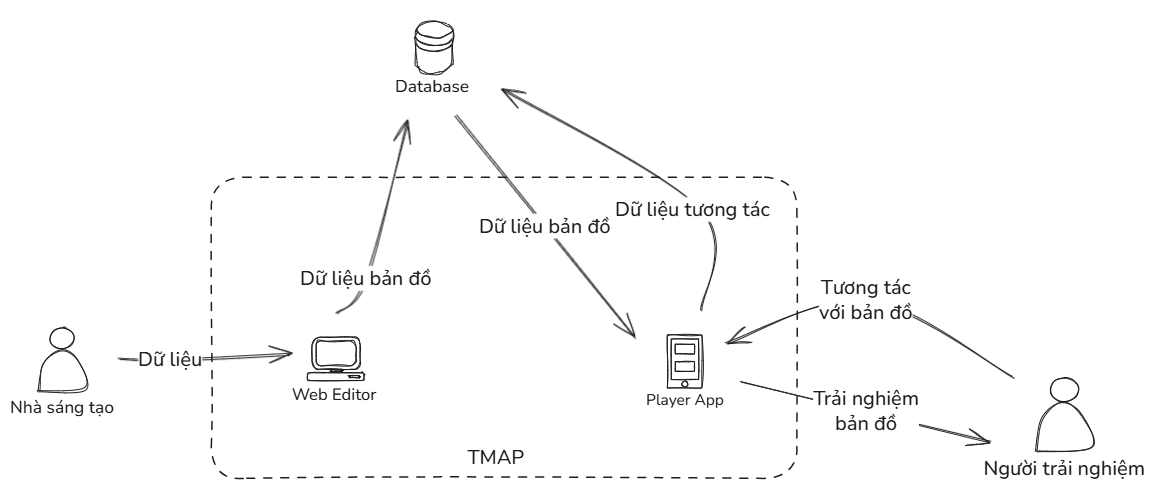
\includegraphics[width=0.9\textwidth]{dataflow.png}
    \caption{Sơ đồ Luồng Dữ liệu trong hệ thống TMAP}
    \label{fig:LuongDuLieuTMAP}
\end{figure}

\subsection{Thiết kế Cơ sở Dữ liệu}

TMAP sử dụng chung cơ sở dữ liệu với hệ thống chung Trealet, với các tác vụ được thực hiện tập trung trên 3 bảng \texttt{au\_trealets}, \texttt{au\_users} và \texttt{au\_user\_to\_trealet}. Bảng \texttt{au\_trealets} lưu thông tin các bản đồ, \texttt{au\_users} lưu thông tin người dùng, và \texttt{au\_user\_to\_trealet} lưu thông tin các tương tác của người dùng với bản đồ. Mối quan hệ giữa các bảng được miêu tả trong \figurename~\ref{fig:ERD_TMAP}.

\begin{figure}[h]
    \centering
    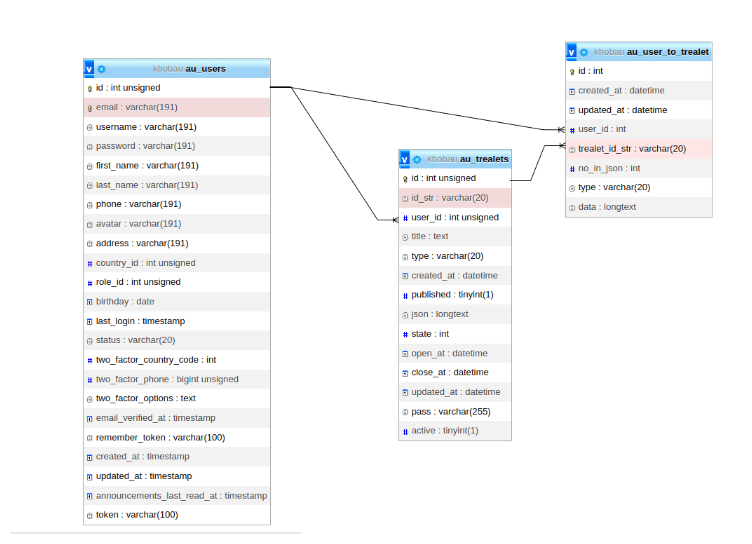
\includegraphics[width=0.9\textwidth]{erd.png}
    \caption{Mô hình Quan hệ Thực thể (ERD) của TMAP Service}
    \label{fig:ERD_TMAP}
\end{figure}

\section{Thiết kế Giao diện và Triển khai}

\subsection{Thiết kế Giao diện Trình biên soạn Web (Editor)}

Trình biên soạn Web được phát triển nhằm mục tiêu đơn giản hóa quy trình số hóa di sản. Giao diện được chia thành hai khu vực chính: khu vực \textbf{Quản lý thông tin chung} (tên Map, mô tả) và khu vực \textbf{Thiết kế bản đồ} (Map Design). Khu vực thiết kế bản đồ là một giao diện đồ họa tích hợp Google Maps, cho phép người dùng nhấp chuột để chọn vị trí, sau đó điền thông tin chi tiết (nội dung, thứ tự, tương tác) vào các form bên cạnh. Việc sử dụng giao diện thân thiện giúp người dùng không có chuyên môn lập trình vẫn có thể dễ dàng tạo ra các Map trải nghiệm có cấu trúc.

\subsection{Thiết kế Giao diện Ứng dụng trải nghiệm di động (Player)}

Ứng dụng trải nghiệm di động được thiết kế để tối ưu hóa sự tương tác và khả năng định vị trên thực địa. Giao diện Player bao gồm các màn hình chính sau:

\begin{enumerate}
    \item \textbf{Màn hình Danh sách Map:} Hiển thị các Map đã xuất bản dưới dạng thẻ (card view) với thông tin tóm tắt và ảnh đại diện, tích hợp chức năng tìm kiếm và phân loại.
    \item \textbf{Màn hình Trải nghiệm Bản đồ:} Đây là màn hình cốt lõi, hiển thị bản đồ với vị trí hiện tại của du khách và các POI. Các POI được đánh số thứ tự rõ ràng. Ứng dụng cung cấp các chỉ dẫn trực quan, ví dụ: các điểm đã hoàn thành được đổi màu để định hướng du khách.
    \item \textbf{Màn hình Tương tác:} Màn hình này được kích hoạt khi du khách đã tiếp cận POI. Giao diện sẽ hiển thị các yêu cầu tương tác (ví dụ: một câu hỏi trắc nghiệm, hoặc nút chụp ảnh/ghi âm) theo cấu hình đã được tạo trên Editor.
\end{enumerate}
Các thiết kế giao diện minh họa chi tiết được trình bày trong \figurename~\ref{fig:GiaoDienEditor} và \figurename~\ref{fig:GiaoDienPlayer}.

% Chừa chỗ cho Hình Giao Diện Editor
% \begin{figure}[h]
%     \centering
%     \caption{Mô phỏng Giao diện Trình biên soạn Web}
%     \label{fig:GiaoDienEditor}
%     \includegraphics[width=0.9\textwidth]{Hinh_Giao_Dien_Editor.png}
% \end{figure}

% Chừa chỗ cho Hình Giao Diện Player
% \begin{figure}[h]
%     \centering
%     \caption{Mô phỏng Giao diện Ứng dụng trải nghiệm di động}
%     \label{fig:GiaoDienPlayer}
%     \includegraphics[width=0.9\textwidth]{Hinh_Giao_Dien_Player.png}
% \end{figure}

\subsection{Triển khai và Tích hợp Hệ thống}

Quá trình triển khai được thực hiện theo nguyên tắc của quy trình DevOps, sử dụng Docker để đóng gói các Microservices của TMAP.
\begin{enumerate}
    \item \textbf{Triển khai Backend và Editor:} Được xây dựng bằng Laravel, hệ thống API được triển khai trên môi trường máy chủ để xử lý các yêu cầu HTTP và tương tác với MySQL database.
    \item \textbf{Triển khai Mobile Player:} Ứng dụng di động được xây dựng bằng Flutter/Dart. Mã nguồn được biên dịch ra các tệp tin cài đặt cho Android và iOS, sẵn sàng cho việc phân phối.
    \item \textbf{Tích hợp API:} Thành phần Player sử dụng các thư viện HTTP để tiêu thụ các RESTful API do TMAP Service cung cấp, đảm bảo khả năng đồng bộ dữ liệu theo thời gian thực.
\end{enumerate}
Quá trình này đảm bảo tính nhất quán, khả năng tái sử dụng và mở rộng, đồng thời giảm thiểu lỗi khi tích hợp TMAP vào nền tảng chung Trealet.